\documentclass{beamer}

\usetheme{Boadilla}


\usepackage{tikz}
\usepackage{pgfplots}
\usepgfplotslibrary{fillbetween}
\usetikzlibrary{arrows.meta, automata, positioning, quotes}
\usepackage[T1]{fontenc}


\title{\textbf{Towards a Better Understanding of Internet Protocol Standardization}}

\subtitle{An Analysis of the IETF Email Archives\\A master thesis presentation}

\author{Cezary Radoslaw Jaskula}


\institute{University of Oslo}

\date{June 18, 2021}


\begin{document}

\frame{\titlepage}



\begin{frame}
\frametitle{The goal of this project }
To develop methods and tools that will allow us to analyze the decision-making contained within the IETF email archives.\\
\bigskip


\end{frame}


\begin{frame}
\frametitle{Why ?}

The process that leads to the creation of these standards is not frequently undergoing a systematic analysis. 


\end{frame}


\begin{frame}
\frametitle{How ?}
By parsing the email archives from their raw state and ingesting the data into a customized, semi-structured, full-text database building on the Apache Solr framework. 

\end{frame}





\begin{frame}
\frametitle{The IETF}

\begin{itemize}

\item Internet Engineering Task Force
\item Participants not members
\item Working Groups
\item Mailing lists
\item Meetings three times a year
\item Drafts - last only 185 days
\item RFCs - the finished product

\item The tools team


\end{itemize}

\end{frame}


\begin{frame}
\frametitle{Toolchain}
    \begin{enumerate}
    \item Email archives (mbox files)
\item Cleanarch 
\item Parser
\item Solr 
\item Queries (statistics)
\item Web scraper
    \end{enumerate}
\end{frame}



\begin{frame}
\frametitle{The email archives }

\begin{itemize}

\item Saved in mbox format
\item Mbox format commonly used in unix distro
\item Inherently flawed in the way messages are stored
\item Solved by cleanarch


\end{itemize}
\end{frame}

\begin{frame}

\frametitle{Cleanarch}

\begin{itemize}
\item Script created to solve the mbox separator problem\\
\item Uses Python 2
\item Modified to run outside of the Mailman framework\\
\item Uses "|" instead of ">"\\
\item Used in this project to clean the mbox files\\

\item Error = the presence of a default value in a mandatory field \\
\begin{itemize}

\item From

\item To

\item Date

\end{itemize}
\item Heavily reduced the error rate in the final database\\


\end{itemize}

\end{frame}




\begin{frame}

\frametitle{Cleanarch results}

\begin{table}

 \begin{tabular}{|c | c | c | c | c|}
 \hline
 Error combination & Before & After & Decrease \\ [0.5ex]
 \hline\hline
ALL & 38809 & 20992 & 45.89\%\\
\hline
From + Date + Dest & 6934 & 443 & 93.61\%\\
\hline
From + Date & 29 & 22 & 24.13\%\\
\hline
From + Dest & 157 & 157 & 0\%\\
\hline
Date + Dest & 44 & 44 & 0\%\\
\hline
From & 89 & 89 & 0\%\\
\hline
Date &  12736 & 12736 & 0\%\\
\hline
Dest &  18820 & 7501 & 64.14\%\\
\hline

\end{tabular}

\end{table}

Clean files produce 2893656 documents

\end{frame}


\begin{frame}

\frametitle{File categories}

\begin{itemize}

\item 3 categories

\begin{itemize}

\item mbox

\item possibly mbox

\item not mbox

\end{itemize}

\item Much higher error rate in Category 2

\item Category 2 cleaned and added to the database

\item Eliminated 1096 out of 11219 errors

\item Clean category 2 files produce 106030 documents



\item Content field made longer

\end{itemize}

\end{frame}

\begin{frame}

\frametitle{Solr}

\begin{itemize}

\item Core

\item Schema

\begin{itemize}
\item Defines fields and their datatype
\item Affects queries and results
\item Tokenizers 
\end{itemize}

\item Date field \\

\item Fields with name and address pairs split into 3

\begin{itemize}
\item Address
\item Name
\item Raw 
\end{itemize}


\end{itemize}

\end{frame}




\begin{frame}
\frametitle{Parser}

\begin{itemize}

\item Python\\
\item mailbox 

\begin{itemize}

\item Allowes to iterate over messages in a mbox file \\

\end{itemize}

\item email.utils

\begin{itemize}

\item Extract information from fields\\

\item Used to extract names and addresses\\

\end{itemize}


\item Pysolr

\begin{itemize}

\item Communication with the Solr instance\\

\end{itemize}



\item Default value if extraction fails


\end{itemize}




\end{frame}



\begin{frame}
\frametitle{Faceting}

\begin{itemize}

\item Query augmentation option\\
\item Calculations done based on results set of query 
\item Counts tokens in a given field 
\item Used to calculate statistics\\
\item Automatically sorted in decreasing order
\item Example

\begin{itemize}

\item query = *:*
\item facet.field = From-address


\end{itemize}

\end{itemize}

\end{frame}




\begin{frame}
\begin{center}
 \begin{tabular}{|c | c | c|}
 \hline
Ranking & address & Value \\ [0.5ex]
 \hline\hline
 1 & black\_david@emc.com & 14365\\
  \hline
 2 & brian.e.carpenter@gmail.com & 13491\\
  \hline
 3 & marcelrf@bellsouth.net & 11485\\
  \hline
 4 & julian.reschke@gmx.de & 10500\\
  \hline
 5 & christer.holmberg@ericsson.com & 10230\\
  \hline
 6 & stephen.farrell@cs.tcd.ie & 8567\\
  \hline
 7 & martin.thomson@gmail.com & 8522\\
  \hline
 8 & cabo@tzi.org & 7915\\
  \hline
 9 & dromasca@avaya.com & 7606\\
  \hline
 10 & jari.arkko@piuha.net & 7482\\
  \hline
 11 & j.schoenwaelder@jacobs-university.de & 7306\\
  \hline
 12 & paul.hoffman@vpnc.org & 7108\\
  \hline
 13 & mcr+ietf@sandelman.ca & 7101\\
  \hline
 14 & mnot@mnot.net & 7043\\
  \hline
 15 & adrian@olddog.co.uk & 6811\\
  \hline
\end{tabular}
\end{center}

\end{frame}


\begin{frame}


\begin{center}
 \begin{tabular}{|c | c | c|}
 \hline
Ranking & address & Value \\ [0.5ex]
 \hline\hline
1 & ietf & 134157\\
\hline
2 & i-d-announce & 103544\\
\hline
3 & quic-issues & 54104\\
\hline
4 & v6ops & 44450\\
\hline
5 & ips & 40603\\
\hline
6 & avt & 40454\\
\hline
7 & dmarc-report & 40007\\
\hline
8 & ipv6 & 38591\\
\hline
9 & httpbisa & 38133\\
\hline
10 & mobileip & 37475\\
\hline
\end{tabular}


\end{center}



\end{frame}


\begin{frame}

\begin{figure}

\frametitle{Messages sent to all mailing lists per year}

\hspace*{-0.3cm}
\centering
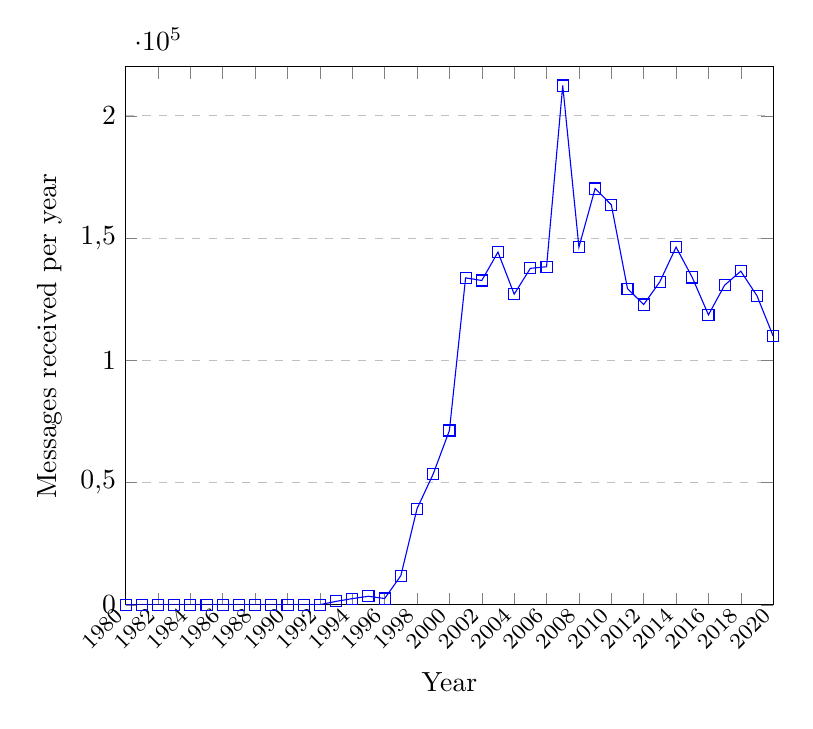
\begin{tikzpicture}
\begin{axis}[
     /pgf/number format/.cd,
     use comma,
    1000 sep={},
    xlabel={Year},
    scale = 1.2,
    ylabel={Messages received per year},
    xmin=1980, xmax=2020,
    ymin=0, ymax=220000,
    xtick={1980,1982,1984,1986,1988,1990,1992 ,1994,1996,1998,2000,2002,2004,2006,2008,2010,2012,2014,2016,2018,2020},
    x tick label style={font=\footnotesize,rotate=45, anchor=east},
    legend pos=north west,
    ymajorgrids=true,
    grid style=dashed,
]
\addplot[
    color=blue,
    mark=square,
    ]
    coordinates {(1980,44)(1981,1)(1982,0)(1983,0)(1984,1)(1985,1)(1986,0)(1987,17)(1988,25)(1989,2)(1990,14)(1991,2)(1992,90)(1993,1429)(1994,2548)(1995,3513)(1996,2586)(1997,11951)(1998,39318)(1999,53552)(2000,71311)(2001,133723)(2002,132650)(2003,144272)(2004,127047)(2005,137615)(2006,138269)(2007,212367)(2008,146271)(2009,170249)(2010,163604)(2011,129325)(2012,122814)(2013,132127)(2014,146299)(2015,133892)(2016,118598)(2017,130735)(2018,136456)(2019,126353)(2020,109885)

    };
 
    
\end{axis}
\end{tikzpicture}
\end{figure}

\end{frame}


\begin{frame}
\frametitle{Crosstalk}


\begin{figure}[H]
\hspace*{-0.4cm}
\centering
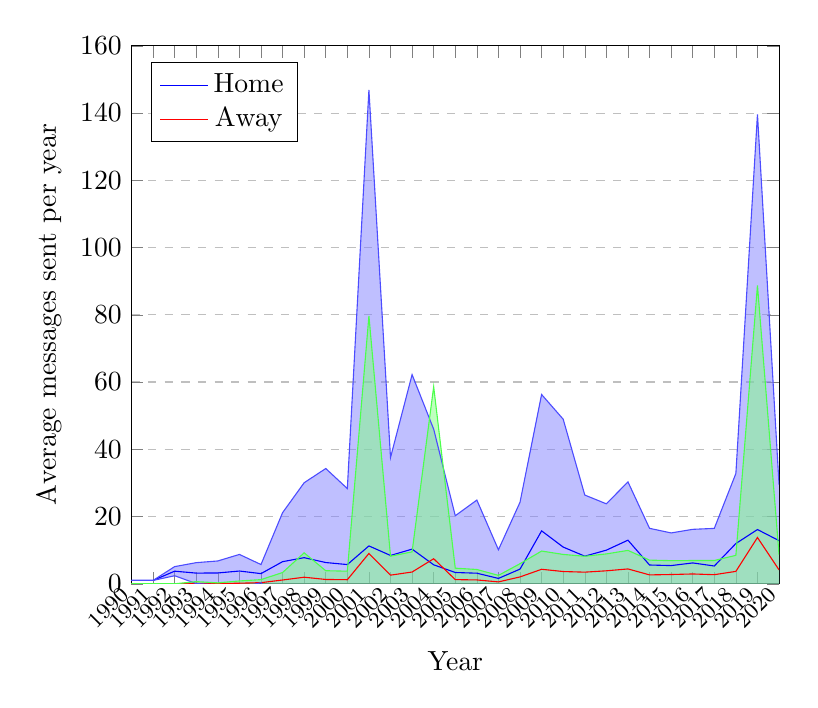
\begin{tikzpicture}
\begin{axis}[
     /pgf/number format/.cd,
     use comma,
    1000 sep={},
    xlabel={Year},
    ylabel={Average messages sent  per year},
    scale=1.2,
    xmin=1990, xmax=2020,
    ymin=0, ymax=160,
    xtick={1980,1981,1982,1983 ,1984,1985,1986,1987,1988,1989,1990,1991,1992,1993 ,1994,1995,1996,1997,1998,1999,2000,2001,2002,2003,2004,2005,2006,2007,2008,2009,2010,2011,2012,2013,2014,2015,2016,2017,2018,2019,2020},
    x tick label style={font=\footnotesize,rotate=45, anchor=east},
    legend pos=north west,
    ymajorgrids=true,
    grid style=dashed,
]

\addplot[color=blue] coordinates {
(1990,1.0)(1991,1.0)(1992,3.75)(1993,3.1767441860465118)(1994,3.2215108834827144)(1995,3.794582392776524)(1996,3.0233766233766235)(1997,6.578186596583443)(1998,7.770768431983385)(1999,6.319893270085977)(2000,5.717015653588128)(2001,11.262751159196291)(2002,8.427462309289519)(2003,10.305207999144477)(2004,5.646533490011751)(2005,3.3577649785769474)(2006,3.1498165378063163)(2007,1.59815093300574)(2008,4.364152269987947)(2009,15.736083357122466)(2010,10.915165411071078)(2011,8.21152052238806)(2012,10.003825310806503)(2013,12.969667318982388)(2014,5.586557742294838)(2015,5.412939898018892)(2016,6.204527799356343)(2017,5.288224799286351)(2018,11.974908318857363)(2019,16.13351842503786)(2020,12.825660825660826)};\addlegendentry{Home}

\addplot[color=red] coordinates {
(1990,0.0)(1991,0.0)(1992,0.0)(1993,0.14883720930232558)(1994,0.05377720870678617)(1995,0.17474633596392333)(1996,0.33548387096774196)(1997,1.1273499090357793)(1998,1.9550683742131538)(1999,1.2872072525812137)(2000,1.2140451330414281)(2001,9.021306252489047)(2002,2.568643056108237)(2003,3.502071563088512)(2004,7.449174259681094)(2005,1.2439513022037294)(2006,1.1430809994586741)(2007,0.5591591085652243)(2008,2.042687044606362)(2009,4.314027213792121)(2010,3.646523279970671)(2011,3.458050605618619)(2012,3.861317365269461)(2013,4.416018533840807)(2014,2.6466901505100875)(2015,2.7566333519354673)(2016,2.921702481301199)(2017,2.706214990664177)(2018,3.688228299643282)(2019,13.768576742538304)(2020,4.125013612109332)};
\addlegendentry{Away}

\addplot[name path=us_top,color=blue!70] coordinates {
(1990,1.0)(1991,1.0)(1992,5.105928341272748)(1993,6.28361648619883)(1994,6.7883537893802135)(1995,8.730361095096416)(1996,5.724601647346882)(1997,21.145462195101327)(1998,30.053087109158664)(1999,34.277924047771705)(2000,28.318978030396675)(2001,146.88319352455096)(2002,37.53355750602556)(2003,62.20502422620849)(2004,45.986816318787)(2005,20.23605884444096)(2006,24.894047726099984)(2007,10.111129539206186)(2008,24.2544293769453)(2009,56.29186263021945)(2010,48.94787263164849)(2011,26.391619081263798)(2012,23.780642131463424)(2013,30.309200413817745)(2014,16.494779130474228)(2015,15.122898278554313)(2016,16.19405185273626)(2017,16.473520184977065)(2018,32.80416142798326)(2019,139.62310539455174)(2020,29.472311504750902)};


\addplot[name path=us_down,color=blue!70] coordinates {
(1990,1.0)(1991,1.0)(1992,2.3940716587272517)(1993,0.06987188589419357)(1994,-0.3453320224147842)(1995,-1.141196309543369)(1996,0.3221515994063653)(1997,-7.989089001934442)(1998,-14.511550245191895)(1999,-21.63813750759975)(2000,-16.88494672322042)(2001,-124.35769120615839)(2002,-20.67863288744652)(2003,-41.59460822791953)(2004,-34.6937493387635)(2005,-13.520528887287066)(2006,-18.59441465048735)(2007,-6.914827673194705)(2008,-15.526124836969405)(2009,-24.819695915974513)(2010,-27.117541809506328)(2011,-9.968578036487678)(2012,-3.772991509850417)(2013,-4.369865775852968)(2014,-5.32166364588455)(2015,-4.2970184825165285)(2016,-3.7849962540235724)(2017,-5.8970705864043635)(2018,-8.85434479026853)(2019,-107.35606854447602)(2020,-3.82098985342925)};


\addplot[blue!50,fill opacity=0.5] fill between[of=us_top and us_down];




\addplot[name path=div_top,color=green!70] coordinates {
(1990,0.0)(1991,0.0)(1992,0.0)(1993,0.6444425583245577)(1994,0.2813157811106731)(1995,0.8412069594535859)(1996,1.2358017706562239)(1997,3.353880239704391)(1998,9.203219187215307)(1999,3.888697199732486)(2000,3.747244603125343)(2001,79.68059769123096)(2002,8.206458157710884)(2003,9.496109236286902)(2004,58.61577301492333)(2005,4.644492135426392)(2006,4.252095224622129)(2007,2.502703694293124)(2008,5.973824939305885)(2009,9.739015781751037)(2010,8.732101165066247)(2011,8.179219588007452)(2012,8.885057628539831)(2013,9.933899481495201)(2014,7.0365925217947956)(2015,6.886481866327898)(2016,6.916233286047339)(2017,6.922928939517584)(2018,8.46461692139536)(2019,88.76168041553137)(2020,8.661465861203498)};


\addplot[name path=div_down,color=green!70] coordinates {
(1990,0.0)(1991,0.0)(1992,0.0)(1993,-0.3467681397199065)(1994,-0.1737613636971008)(1995,-0.4917142875257393)(1996,-0.5648340287207401)(1997,-1.0991804216328327)(1998,-5.293082438788999)(1999,-1.3142826945700588)(2000,-1.3191543370424865)(2001,-61.63798518625287)(2002,-3.06917204549441)(2003,-2.491966110109878)(2004,-43.71742449556114)(2005,-2.156589531018933)(2006,-1.9659332257047806)(2007,-1.3843854771626751)(2008,-1.8884508500931605)(2009,-1.110961354166795)(2010,-1.4390546051249045)(2011,-1.263118376770215)(2012,-1.16242289800091)(2013,-1.1018624138135866)(2014,-1.7432122207746206)(2015,-1.3732151624569635)(2016,-1.07282832344494)(2017,-1.5104989581892299)(2018,-1.0881603221087963)(2019,-61.22452693045477)(2020,-0.4114386369848333)};


\addplot[green!50,fill opacity=0.5] fill between[of=div_top and div_down];





\end{axis}
\end{tikzpicture}
\caption{Messages sent to an address's home mailing list, as well as any other mailing lists that are not their home. Blue and green shaded areas show the standard deviation for the "Home" and "Away" cases, respectively.}
\end{figure}



\end{frame}


\begin{frame}
\frametitle{Conversation tracking}

\begin{itemize}

\item In-reply-to-field\\
\item Messages as nodes\\
\item Parent - child relation\\
\item Incorrect dates 
\item Relations mapped and represented as bidirectional graphs\\

\item 2 cores 
\begin{itemize}

\item Nodes
\item Graphs

\end{itemize}

\item Graphs are conversations




\end{itemize}

\end{frame}


\begin{frame}
\frametitle{Resulting graphs}



\begin{figure}[H]
\hspace*{-0.5cm}
\centering
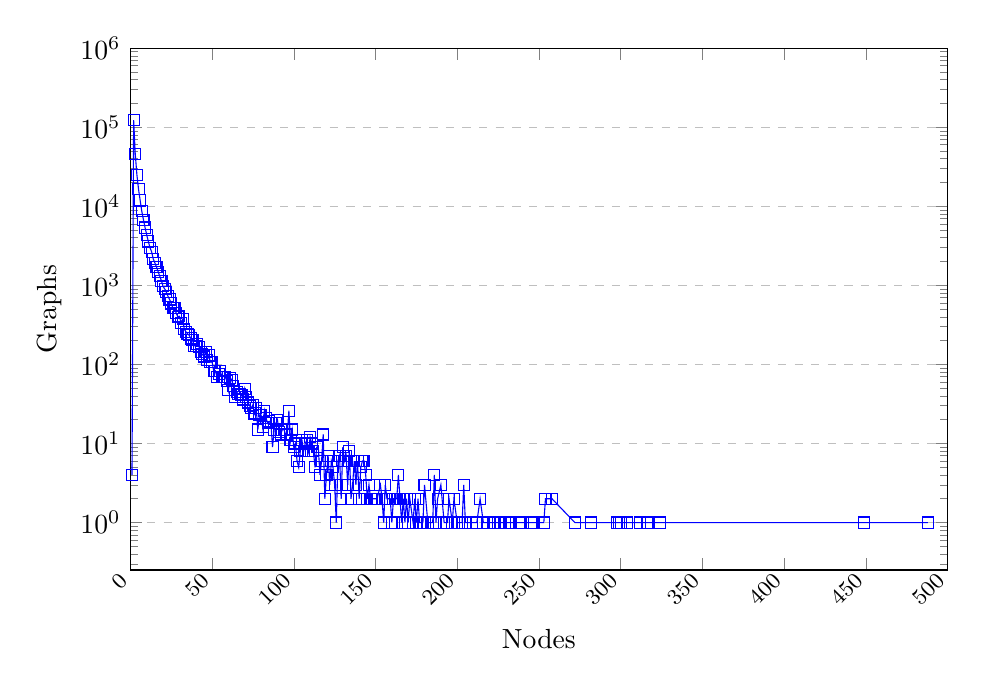
\begin{tikzpicture}
\begin{axis}[
     /pgf/number format/.cd,
     use comma,
    1000 sep={},
    width=8.5cm, height=6cm, 
    xlabel={Nodes},
    ylabel={Graphs},
    scale=1.5,
    xmin=0, xmax=500,
    ymode=log,
    ymin=0, ymax=1e6,
    x tick label style={font=\footnotesize,rotate=45, anchor=east},
    legend pos=north west,
    ymajorgrids=true,
    grid style=dashed,
]
\addplot[
    color=blue,
    mark=square,
    ]
    coordinates {
(1,4)(2,123015)(3,45537)(4,25069)(5,16409)(6,11851)(7,8645)(8,6758)(9,5387)(10,4355)(11,3593)(12,2994)(13,2666)(14,2161)(15,1926)(16,1707)(17,1483)(18,1304)(19,1148)(20,971)(21,903)(22,823)(23,728)(24,663)(25,591)(26,513)(27,514)(28,448)(29,402)(30,406)(31,337)(32,373)(33,280)(34,258)(35,245)(36,234)(37,213)(38,203)(39,173)(40,171)(41,183)(42,167)(43,142)(44,135)(45,126)(46,144)(47,113)(48,130)(49,107)(50,108)(51,82)(52,83)(53,70)(54,76)(55,83)(56,70)(57,70)(58,70)(59,62)(60,47)(61,68)(62,64)(63,53)(64,39)(65,45)(66,42)(67,42)(68,41)(69,36)(70,49)(71,39)(72,33)(73,30)(74,28)(75,31)(76,24)(77,28)(78,15)(79,23)(80,23)(81,16)(82,26)(83,21)(84,18)(85,19)(86,18)(87,9)(88,15)(89,18)(90,20)(91,14)(92,13)(93,15)(94,15)(95,13)(96,13)(97,26)(98,11)(99,15)(100,9)(101,10)(102,6)(103,5)(104,8)(105,11)(106,8)(107,10)(108,11)(109,8)(110,12)(111,10)(112,8)(113,5)(114,9)(115,9)(116,4)(117,6)(118,13)(119,2)(120,4)(121,7)(122,3)(123,6)(124,5)(125,3)(126,1)(127,6)(128,7)(129,2)(130,9)(131,6)(132,7)(133,3)(134,8)(135,2)(136,3)(137,6)(138,3)(139,6)(140,2)(141,5)(142,6)(143,6)(144,4)(145,2)(146,3)(147,2)(148,2)(149,2)(150,2)(151,2)(153,3)(154,2)(155,1)(156,3)(157,2)(159,2)(160,1)(161,2)(162,2)(163,2)(164,4)(165,2)(166,1)(167,2)(168,1)(169,2)(170,1)(171,2)(173,1)(174,2)(175,1)(176,2)(177,1)(178,1)(179,1)(180,3)(182,1)(185,1)(186,4)(187,1)(188,2)(190,3)(192,1)(193,1)(194,1)(195,2)(197,1)(198,2)(200,1)(201,1)(203,1)(204,3)(205,1)(212,1)(214,2)(216,1)(218,1)(222,1)(223,1)(226,1)(227,1)(229,1)(232,1)(233,1)(238,1)(245,1)(246,1)(247,1)(253,1)(254,2)(258,2)(272,1)(282,1)(298,1)(299,1)(300,1)(304,1)(312,1)(316,1)(317,1)(324,1)(449,1)(488,1)
    };
  
    
\end{axis}
\end{tikzpicture}
\caption{The number of graphs of a certain length contained in the database.}
\end{figure}

\end{frame}


\begin{frame}
\frametitle{High level conversation tracking}

\begin{enumerate}
\item Execute query on the “Subject” and “Content” fields
\item Identify the graphs the nodes in the results set belong to 
\item Fetch graphs nodes from Solr
\item For each graph, set the nodes from the query results set as “targets”
\item For each target, try and find a path to any of the other targets
\item For each path found, save the nodes in it in a set 
\item See if any paths have common nodes, if yes, merge them 
\item Finally, for each result set, order the nodes by date


\end{enumerate}


\end{frame}


\begin{frame}

\frametitle{Tracking "Last call"}

Amount of conversations found = 23254\\
Average length = 4.567\\
Standard deviation = 6.931\\

\end{frame}




\begin{frame}

\frametitle{"Last call"}
\begin{figure}[H]
\hspace*{-0.5cm}
\centering
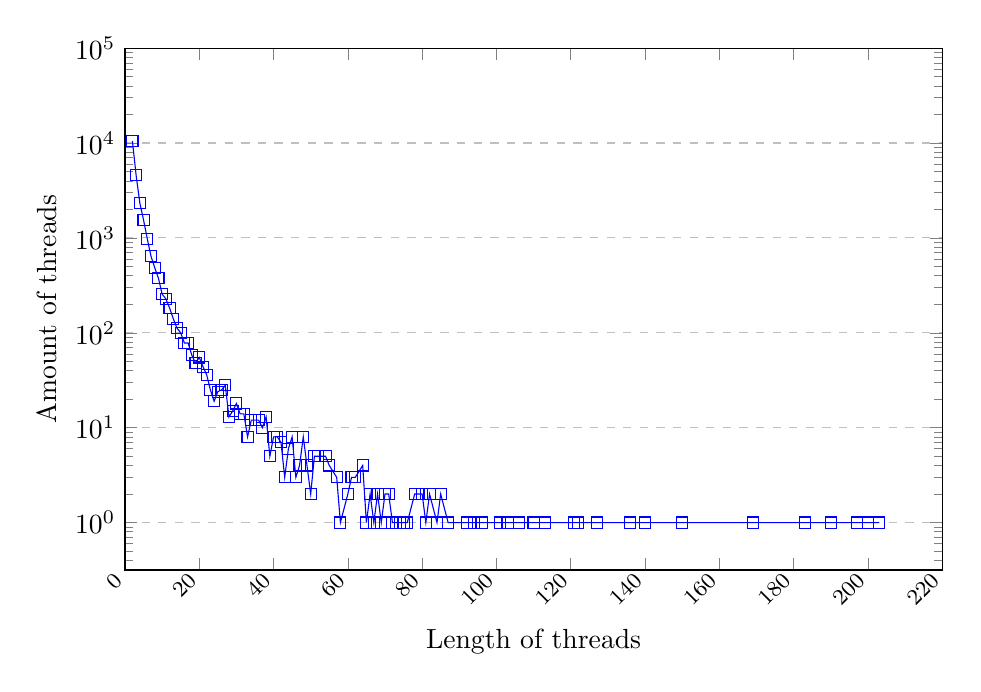
\begin{tikzpicture}
\begin{axis}[
     /pgf/number format/.cd,
     use comma,
    1000 sep={},
    width=8.5cm, height=6cm, 
    xlabel={Length of threads},
    ylabel={Amount of threads},
    scale=1.5,
    xmin=0, xmax=220,
    ymode=log,
    ymin=0, ymax=1e5,
    x tick label style={font=\footnotesize,rotate=45, anchor=east},
    legend pos=north west,
    ymajorgrids=true,
    grid style=dashed,
]
\addplot[
    color=blue,
    mark=square,
    ]
    coordinates {
(2,10493)(3,4572)(4,2329)(5,1547)(6,980)(7,643)(8,486)(9,377)(10,256)(11,228)(12,183)(13,141)(14,112)(15,100)(16,78)(17,78)(18,58)(19,48)(20,55)(21,44)(22,36)(23,25)(24,19)(25,24)(26,25)(27,28)(28,13)(29,15)(30,18)(31,14)(32,14)(33,8)(34,12)(35,12)(36,12)(37,10)(38,13)(39,5)(40,8)(41,8)(42,7)(43,3)(44,6)(45,8)(46,3)(47,4)(48,8)(49,4)(50,2)(51,5)(52,5)(54,5)(55,4)(57,3)(58,1)(60,2)(61,3)(62,3)(64,4)(65,1)(66,2)(67,1)(68,2)(69,1)(70,2)(71,2)(72,1)(73,1)(74,1)(75,1)(76,1)(78,2)(80,2)(81,1)(82,2)(84,1)(85,2)(87,1)(92,1)(94,1)(96,1)(101,1)(103,1)(106,1)(110,1)(113,1)(121,1)(122,1)(127,1)(136,1)(140,1)(150,1)(169,1)(183,1)(190,1)(197,1)(200,1)(203,1)
    };
  
    
\end{axis}
\end{tikzpicture}
\end{figure}



\end{frame}


\begin{frame}
\frametitle{"Last call"}
\begin{figure}[H]
\hspace*{-0.5cm}
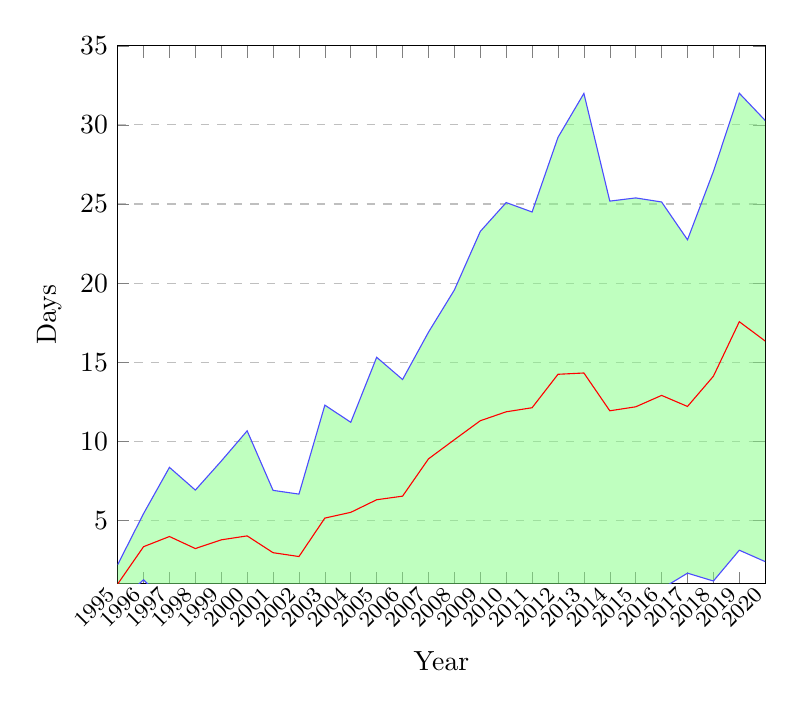
\begin{tikzpicture}
\begin{axis}[
     /pgf/number format/.cd,
     use comma,
    1000 sep={},
    xlabel={Year},
    ylabel={Days},
    scale=1.2,
    xmin=1995, xmax=2020,
    ymin=1, ymax=35,
    xtick={1990,1991,1992,1993 ,1994,1995,1996,1997,1998,1999,2000,2001,2002,2003,2004,2005,2006,2007,2008,2009,2010,2011,2012,2013,2014,2015,2016,2017,2018,2019,2020},
    x tick label style={font=\footnotesize,rotate=45, anchor=east},
    legend pos=north west,
    ymajorgrids=true,
    grid style=dashed,
]


\addplot[color=red] coordinates {
(1995,0.979748185685686)
(1996,3.3429012345679014)
(1997,3.9866254516711828)
(1998,3.225154299672601)
(1999,3.776405873066553)
(2000,4.02591916483315)
(2001,2.9634600215263034)
(2002,2.7208327974965703)
(2003,5.151680933235868)
(2004,5.51441265587782)
(2005,6.310517238834918)
(2006,6.537172986478542)
(2007,8.893092615857064)
(2008,10.10630700420954)
(2009,11.303461541734748)
(2010,11.868171806917212)
(2011,12.125650036251587)
(2012,14.239504293801572)
(2013,14.321117469607993)
(2014,11.932393414500448)
(2015,12.183628837945754)
(2016,12.904897473384315)
(2017,12.205768003481724)
(2018,14.117222824341681)
(2019,17.562622253086417)
(2020,16.339489975512706)
};


\addplot[name path=us_top,color=blue!70] coordinates {
(1995,2.2033788316755683)
(1996,5.433947810341324)
(1997,8.357325582812347)
(1998,6.920828842255933)
(1999,8.752969510473655)
(2000,10.665780562896723)
(2001,6.902625960252331)
(2002,6.666968324256853)
(2003,12.289292381692503)
(2004,11.205850706436934)
(2005,15.313024283461473)
(2006,13.90895723049302)
(2007,16.899437725893648)
(2008,19.568548060956722)
(2009,23.26748289945725)
(2010,25.09324839600957)
(2011,24.49638414760995)
(2012,29.213792496827296)
(2013,31.989865070370776)
(2014,25.184240020644204)
(2015,25.386096980499836)
(2016,25.12911097368187)
(2017,22.741616580912556)
(2018,27.061198354857403)
(2019,32.00310826131279)
(2020,30.280693234138326)
};


\addplot[name path=us_down,color=blue!70] coordinates {
(1995,-0.24388246030419625)
(1996,1.2518546587944792)
(1997,-0.3840746794699821)
(1998,-0.4705202429107307)
(1999,-1.200157764340548)
(2000,-2.613942233230423)
(2001,-0.9757059171997242)
(2002,-1.225302729263713)
(2003,-1.9859305152207671)
(2004,-0.1770253946812952)
(2005,-2.6919898057916383)
(2006,-0.8346112575359337)
(2007,0.8867475058204803)
(2008,0.6440659474623587)
(2009,-0.6605598159877513)
(2010,-1.356904782175146)
(2011,-0.2450840751067762)
(2012,-0.7347839092241522)
(2013,-3.347630131154789)
(2014,-1.3194531916433103)
(2015,-1.0188393046083295)
(2016,0.6806839730867598)
(2017,1.6699194260508907)
(2018,1.1732472938259608)
(2019,3.1221362448600463)
(2020,2.398286716887087)
};



\addplot[green!50,fill opacity=0.5] fill between[of=us_top and us_down];
  
    
\end{axis}
\end{tikzpicture}
\end{figure}


\end{frame}


\begin{frame}

\frametitle{"Last call"}

\begin{figure}[H]
\hspace*{-0.5cm}
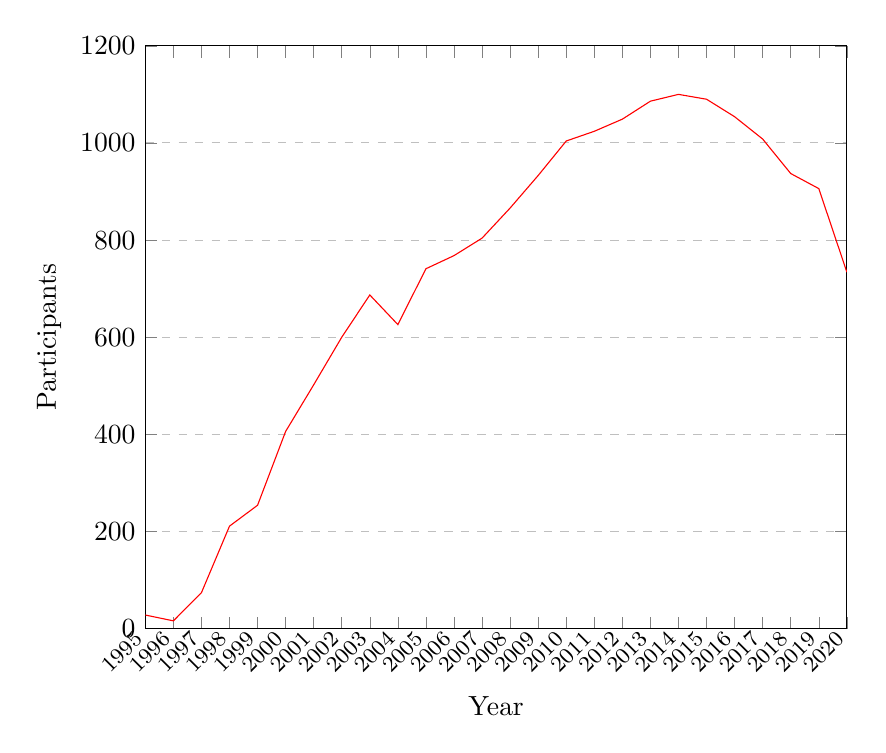
\begin{tikzpicture}
\begin{axis}[
     /pgf/number format/.cd,
     use comma,
    1000 sep={},
    xlabel={Year},
    ylabel={Participants},
    scale=1.3,
    xmin=1995, xmax=2020,
    ymin=0, ymax=1200,
    xtick={1990,1991,1992,1993 ,1994,1995,1996,1997,1998,1999,2000,2001,2002,2003,2004,2005,2006,2007,2008,2009,2010,2011,2012,2013,2014,2015,2016,2017,2018,2019,2020},
    x tick label style={font=\footnotesize,rotate=45, anchor=east},
    legend pos=north west,
    ymajorgrids=true,
    grid style=dashed,
]

\addplot[color=red] coordinates {
(1995,28)
(1996,16)
(1997,74)
(1998,211)
(1999,254)
(2000,406)
(2001,502)
(2002,600)
(2003,687)
(2004,626)
(2005,741)
(2006,768)
(2007,804)
(2008,866)
(2009,933)
(2010,1004)
(2011,1024)
(2012,1049)
(2013,1086)
(2014,1100)
(2015,1090)
(2016,1054)
(2017,1008)
(2018,937)
(2019,906)
(2020,734)
};

    
\end{axis}
\end{tikzpicture}
\end{figure}


\end{frame}


\begin{frame}
\frametitle{Connecting authors to threads}

\begin{itemize}

\item LaTeX .bib file \\
\item IETF datatracker \\
\item RFC ids


\item Web scraper

\begin{itemize}
\item Beautifulsoup
\end{itemize}


\item More addresses from Solr
 

\end{itemize}


\end{frame}

\begin{frame}


\begin{center}
\begin{table}
\centering
 \begin{tabular}{||c | c | c||} 
 \hline
\textit{Ranking} & \textit{Name} & \textit{RFC count} \\ [1ex] 
 \hline\hline
1 & Russ Housley & 96\\
\hline

2 & Donald Eastlake & 95\\
\hline

3 & Keith McCloghrie & 92\\
\hline

4 & Henning Schulzrinne & 90\\
\hline

5 & Hannes Tschofenig & 85\\
\hline

6 & Yakov Rekhter & 78\\
\hline

7 & Jonathan Rosenberg & 72\\
\hline

8 & Adrian Farrel & 71\\
\hline

9 & Paul Hoffman & 70\\
\hline

10 & Gonzalo Camarillo & 70\\
\hline

11 & Marshall Rose & 65\\
\hline

12 & Fred Baker & 65\\
\hline

13 & Alexey Melnikov & 60\\
\hline

14 & John Klensin & 59\\
\hline

15 & Mohamed Boucadair & 54\\
\hline



\end{tabular}

\end{table}
\end{center}


\end{frame}

\begin{frame}



\begin{figure}[H]
\hspace*{-0.5cm}
\centering
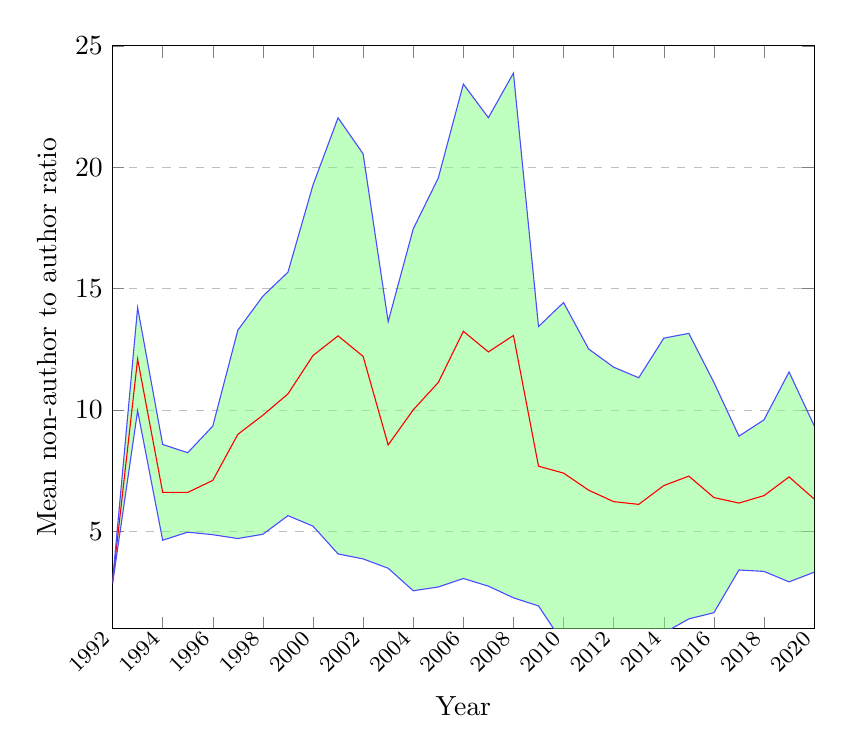
\begin{tikzpicture}
\begin{axis}[
     /pgf/number format/.cd,
     use comma,
    1000 sep={},
    xlabel={Year},
    ylabel={Mean non-author to author ratio},
    scale=1.3,
    xmin=1992, xmax=2020,
    ymin=1, ymax=25,
    xtick={1990,1992 ,1994,1996,1998,2000,2002,2004,2006,2008,2010,2012,2014,2016,2018,2020},
    x tick label style={font=\footnotesize,rotate=45, anchor=east},
    legend pos=north west,
    ymajorgrids=true,
    grid style=dashed,
]

\addplot[color=red] coordinates {
(1992,2.9)
(1993,12.097222222222221)
(1994,6.611111111111111)
(1995,6.607954545454546)
(1996,7.1033333333333335)
(1997,8.999693362193362)
(1998,9.78769077961352)
(1999,10.664359201166064)
(2000,12.244593284056126)
(2001,13.055564425001576)
(2002,12.210450008935537)
(2003,8.563354049280607)
(2004,10.008821808072192)
(2005,11.134915248683626)
(2006,13.24380653561535)
(2007,12.393755244587457)
(2008,13.071598186554604)
(2009,7.687837407471444)
(2010,7.40395625629824)
(2011,6.701907362962169)
(2012,6.228895617775256)
(2013,6.116631190612625)
(2014,6.889446218907785)
(2015,7.279464559055016)
(2016,6.397618233358824)
(2017,6.1701479418746965)
(2018,6.476066768336391)
(2019,7.246304747528565)
(2020,6.3408490306133505)
};


\addplot[name path=us_top,color=blue!70] coordinates {
(1992,2.95)
(1993,14.222108747878021)
(1994,8.582550705436555)
(1995,8.244029626546816)
(1996,9.339552861415891)
(1997,13.289592417850027)
(1998,14.68934910810076)
(1999,15.677528468035145)
(2000,19.269090381135314)
(2001,22.03572505912154)
(2002,20.551150516113015)
(2003,13.641024972940462)
(2004,17.458515460018745)
(2005,19.55566977876152)
(2006,23.423648180945193)
(2007,22.03938950314682)
(2008,23.875424362386084)
(2009,13.440274033428647)
(2010,14.426233144897193)
(2011,12.514855849559396)
(2012,11.765868044614805)
(2013,11.329036622375618)
(2014,12.960319196346916)
(2015,13.158558429103222)
(2016,11.139942441683917)
(2017,8.925841597214218)
(2018,9.59623914170881)
(2019,11.568041320675276)
(2020,9.360110616896266)
};


\addplot[name path=us_down,color=blue!70] coordinates {
(1992,2.8499999999999996)
(1993,9.972335696566422)
(1994,4.639671516785666)
(1995,4.971879464362277)
(1996,4.867113805250776)
(1997,4.709794306536697)
(1998,4.886032451126279)
(1999,5.6511899342969825)
(2000,5.2200961869769404)
(2001,4.0754037908816105)
(2002,3.869749501758058)
(2003,3.485683125620751)
(2004,2.55912815612564)
(2005,2.714160718605733)
(2006,3.0639648902855097)
(2007,2.748120986028095)
(2008,2.2677720107231227)
(2009,1.9354007815142404)
(2010,0.3816793676992889)
(2011,0.888958876364943)
(2012,0.6919231909357073)
(2013,0.9042257588496332)
(2014,0.8185732414686546)
(2015,1.4003706890068113)
(2016,1.6552940250337302)
(2017,3.4144542865351752)
(2018,3.355894394963972)
(2019,2.9245681743818537)
(2020,3.321587444330435)
};




\addplot[green!50,fill opacity=0.5] fill between[of=us_top and us_down];
  
    
\end{axis}
\end{tikzpicture}
\end{figure}


\end{frame}




\begin{frame}
\frametitle{Summary}

\begin{itemize}

\item Email archives parsed and transformed into a Solr compatible format \\
\item Various statistics calculated
\item Relations between messages have been mapped \\
\item Basic thread tracking implemented and working as intended \\
\item Authors and their addresses collected 


\end{itemize}

\end{frame}


\begin{frame}
\frametitle{Conclusion}

\begin{itemize}

\item The IETF is an active forum with many users

\item It is a good place to learn as people talk across mailing lists

\item Both authors and non authors interact and contribute to discussion

\item The “last call” threads are losing participants, and decreasing in length   


\end{itemize}

\end{frame}

\begin{frame}

\frametitle{The end}

\center{Thank you for your time}

\end{frame}


\begin{frame}

\centering
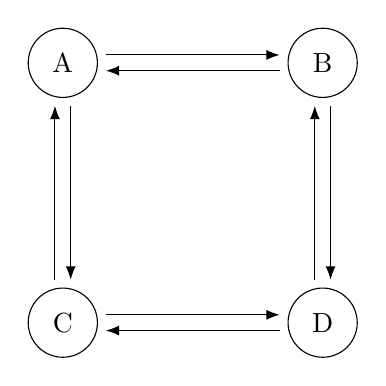
\begin{tikzpicture}[
    shorten < =  1mm, shorten > = 1mm,
node distance = 33mm, on grid, auto,
every path/.style = {-Latex},
sx+/.style = {xshift=1 mm},
sy+/.style = {yshift=1 mm},
sx-/.style = {xshift=-1 mm},
sy-/.style = {yshift=-1 mm},
                    ]
\node[state] (A) {A};
\node[state] (B) [right=of A] {B};
\node[state] (C) [below=of A] {C};
\node[state] (D) [right=of C] {D};
%
\path[->]   ([sy+] A.east)  edge ([sy+] B.west)
            ([sx+] B.south) edge       ([sx+] D.north)
            ([sy-] D.west)  edge       ([sy-] C.east)
            ([sx-] C.north) edge  ([sx-] A.south)
%
            ([sx+] A.south)  edge       ([sx+] C.north)
            ([sy+] C.east)   edge       ([sy+] D.west)
            ([sx-] D.north) edge   ([sx-] B.south)
            ([sy-] B.west)  edge   ([sy-] A.east);
%


\end{tikzpicture}


\end{frame}


\end{document}